%-----------------------Homework------------------------------------
%-------------------Arman Shokrollahi---------------------------------
%---------------------Coding Theory-------------------------------

\documentclass[a4 paper]{article}
% Set target color model to RGB
\usepackage[inner=1.5cm,outer=1.5cm,top=2.5cm,bottom=2.5cm]{geometry}
%\usepackage{setspace}
\usepackage{enumerate}
%\usepackage[rgb]{xcolor}
%\usepackage{verbatim}
\usepackage{amsgen,amsmath,amstext,amsbsy,amsopn,tikz,amssymb,tkz-linknodes}
%%\usepackage{fancyhdr}
\usepackage{bm}
%
%\usepackage[colorlinks=true, urlcolor=blue,  linkcolor=blue, citecolor=blue]{hyperref}
%\usepackage[colorinlistoftodos]{todonotes}
%\usepackage{rotating}
%%\usetikzlibrary{through,backgrounds}
%\hypersetup{%
%pdfauthor={Arman Shokrollahi},%
%pdftitle={Homework},%
%pdfkeywords={Tikz,latex,bootstrap,uncertaintes},%
%pdfcreator={PDFLaTeX},%
%pdfproducer={PDFLaTeX},%
%}
%%\usetikzlibrary{shadows}
%\usepackage[francais]{babel}
%\usepackage{booktabs}
\usepackage{tikz}
\usetikzlibrary{arrows,chains,matrix,positioning,scopes}
%\newcommand{\ra}[1]{\renewcommand{\arraystretch}{#1}}
%
%      \newtheorem{thm}{Theorem}[section]
%      \newtheorem{prop}[thm]{Proposition}
%      \newtheorem{lem}[thm]{Lemma}
%      \newtheorem{cor}[thm]{Corollary}
%      \newtheorem{defn}[thm]{Definition}
%      \newtheorem{rem}[thm]{Remark}
%      \numberwithin{equation}{section}
%
%\newcommand{\bbF}{\mathbb{F}}
%\newcommand{\bbX}{\mathbb{X}}
%\newcommand{\bI}{\mathbf{I}}
%\newcommand{\bX}{\mathbf{X}}
%\newcommand{\bY}{\mathbf{Y}}
%\newcommand{\bepsilon}{\boldsymbol{\epsilon}}
%\newcommand{\balpha}{\boldsymbol{\alpha}}
%\newcommand{\bbeta}{\boldsymbol{\beta}}
%\newcommand{\0}{\mathbf{0}}
%
%\usepackage{xeCJK}
%\setCJKmainfont[BoldFont=STZhongsong, ItalicFont=STKaiti]{STSong}
%\setCJKsansfont[BoldFont=STHeiti]{STXihei}
%\setCJKmonofont{STFangsong}

\newcommand{\spp}{\underline{ \hspace{2cm}}}
\newcommand{\ttt}{\textit}
\newcommand{\vv}{\vskip 1em}
\newcommand{\tab}[1]{\hspace{.2\textwidth}\rlap{#1}}
\newcommand{\an}{$\{a_n\}$}
\linespread{1.2}

\usepackage{courier}
\usepackage{listings}
\usepackage{graphicx}
\usepackage{color}

\definecolor{codegreen}{rgb}{0,0.6,0}
\definecolor{codegray}{rgb}{0.5,0.5,0.5}
\definecolor{codepurple}{rgb}{0.58,0,0.82}
\definecolor{backcolour}{rgb}{0.95,0.95,0.92}

\lstdefinestyle{mystyle}{
	backgroundcolor=\color{backcolour},   
	commentstyle=\color{codegreen},
	keywordstyle=\color{magenta},
	numberstyle=\tiny\color{codegray},
	stringstyle=\color{codepurple},
	basicstyle=\footnotesize\ttfamily,
	breakatwhitespace=false,         
	breaklines=true,                 
	captionpos=b,                    
	keepspaces=true,                 
	numbers=left,                    
	numbersep=5pt,                  
	showspaces=false,                
	showstringspaces=false,
	showtabs=false,                  
	tabsize=4,
	framextopmargin=50pt,frame=bottomline
}
\usepackage{lipsum}
\usepackage{courier}

\lstset{basicstyle=\footnotesize\ttfamily,breaklines=true,commentstyle=\itshape\color{codegreen},numbers=left,numberstyle=\tiny\color{codegray}}
\lstset{framextopmargin=1pt,frame=tblr}
\usepackage{hyperref}
%\lstset{style=mystyle}
\begin{document}
\begin{center}
	\huge\bf Binary Lifting
\end{center}

Binary lifting is a pretty beautiful technique, which has good design stratigies and wide applications. Perhaps mostly popular, it is used to find LCS({\bf lowest common ancestor}) on trees, but it can do more. I think it can help {\bf query paths} on trees.

By DFS, we could maintain the following information:
\begin{enumerate}[(1)]
	\item The level of each node: $L[u]$
	\[
		L[u] = \left\{
			\begin{array}{ll}
			0,&\text{ if }u=root\\
			\\
			L[p(u)]+1,& p(u) \text{ is the parent node of }u.
			\end{array}
		\right.
	\]
	Obviously, we could know the parent of $u$ during the same dfs process.
	\item The $2^i$-th ancestor of $u$: $f[u,i]$. This is the most wonderful part of binary lifting technique. The matrix $f$ has a dimension: $n\times \log n$, so it is both time and memory efficient. We do it by a DP and divide-and-conquer strategy.
	\[
		f[u,i] = \left\{
			\begin{array}{ll}
				p(u),& \text{if }i=0\\
				\\
				f\left[ f[u,i-1],i-1 \right], &\text{otherwise}
			\end{array}
		\right.
	\] 
	Below is a simple example:
	\begin{figure}[!ht]
		\centering
		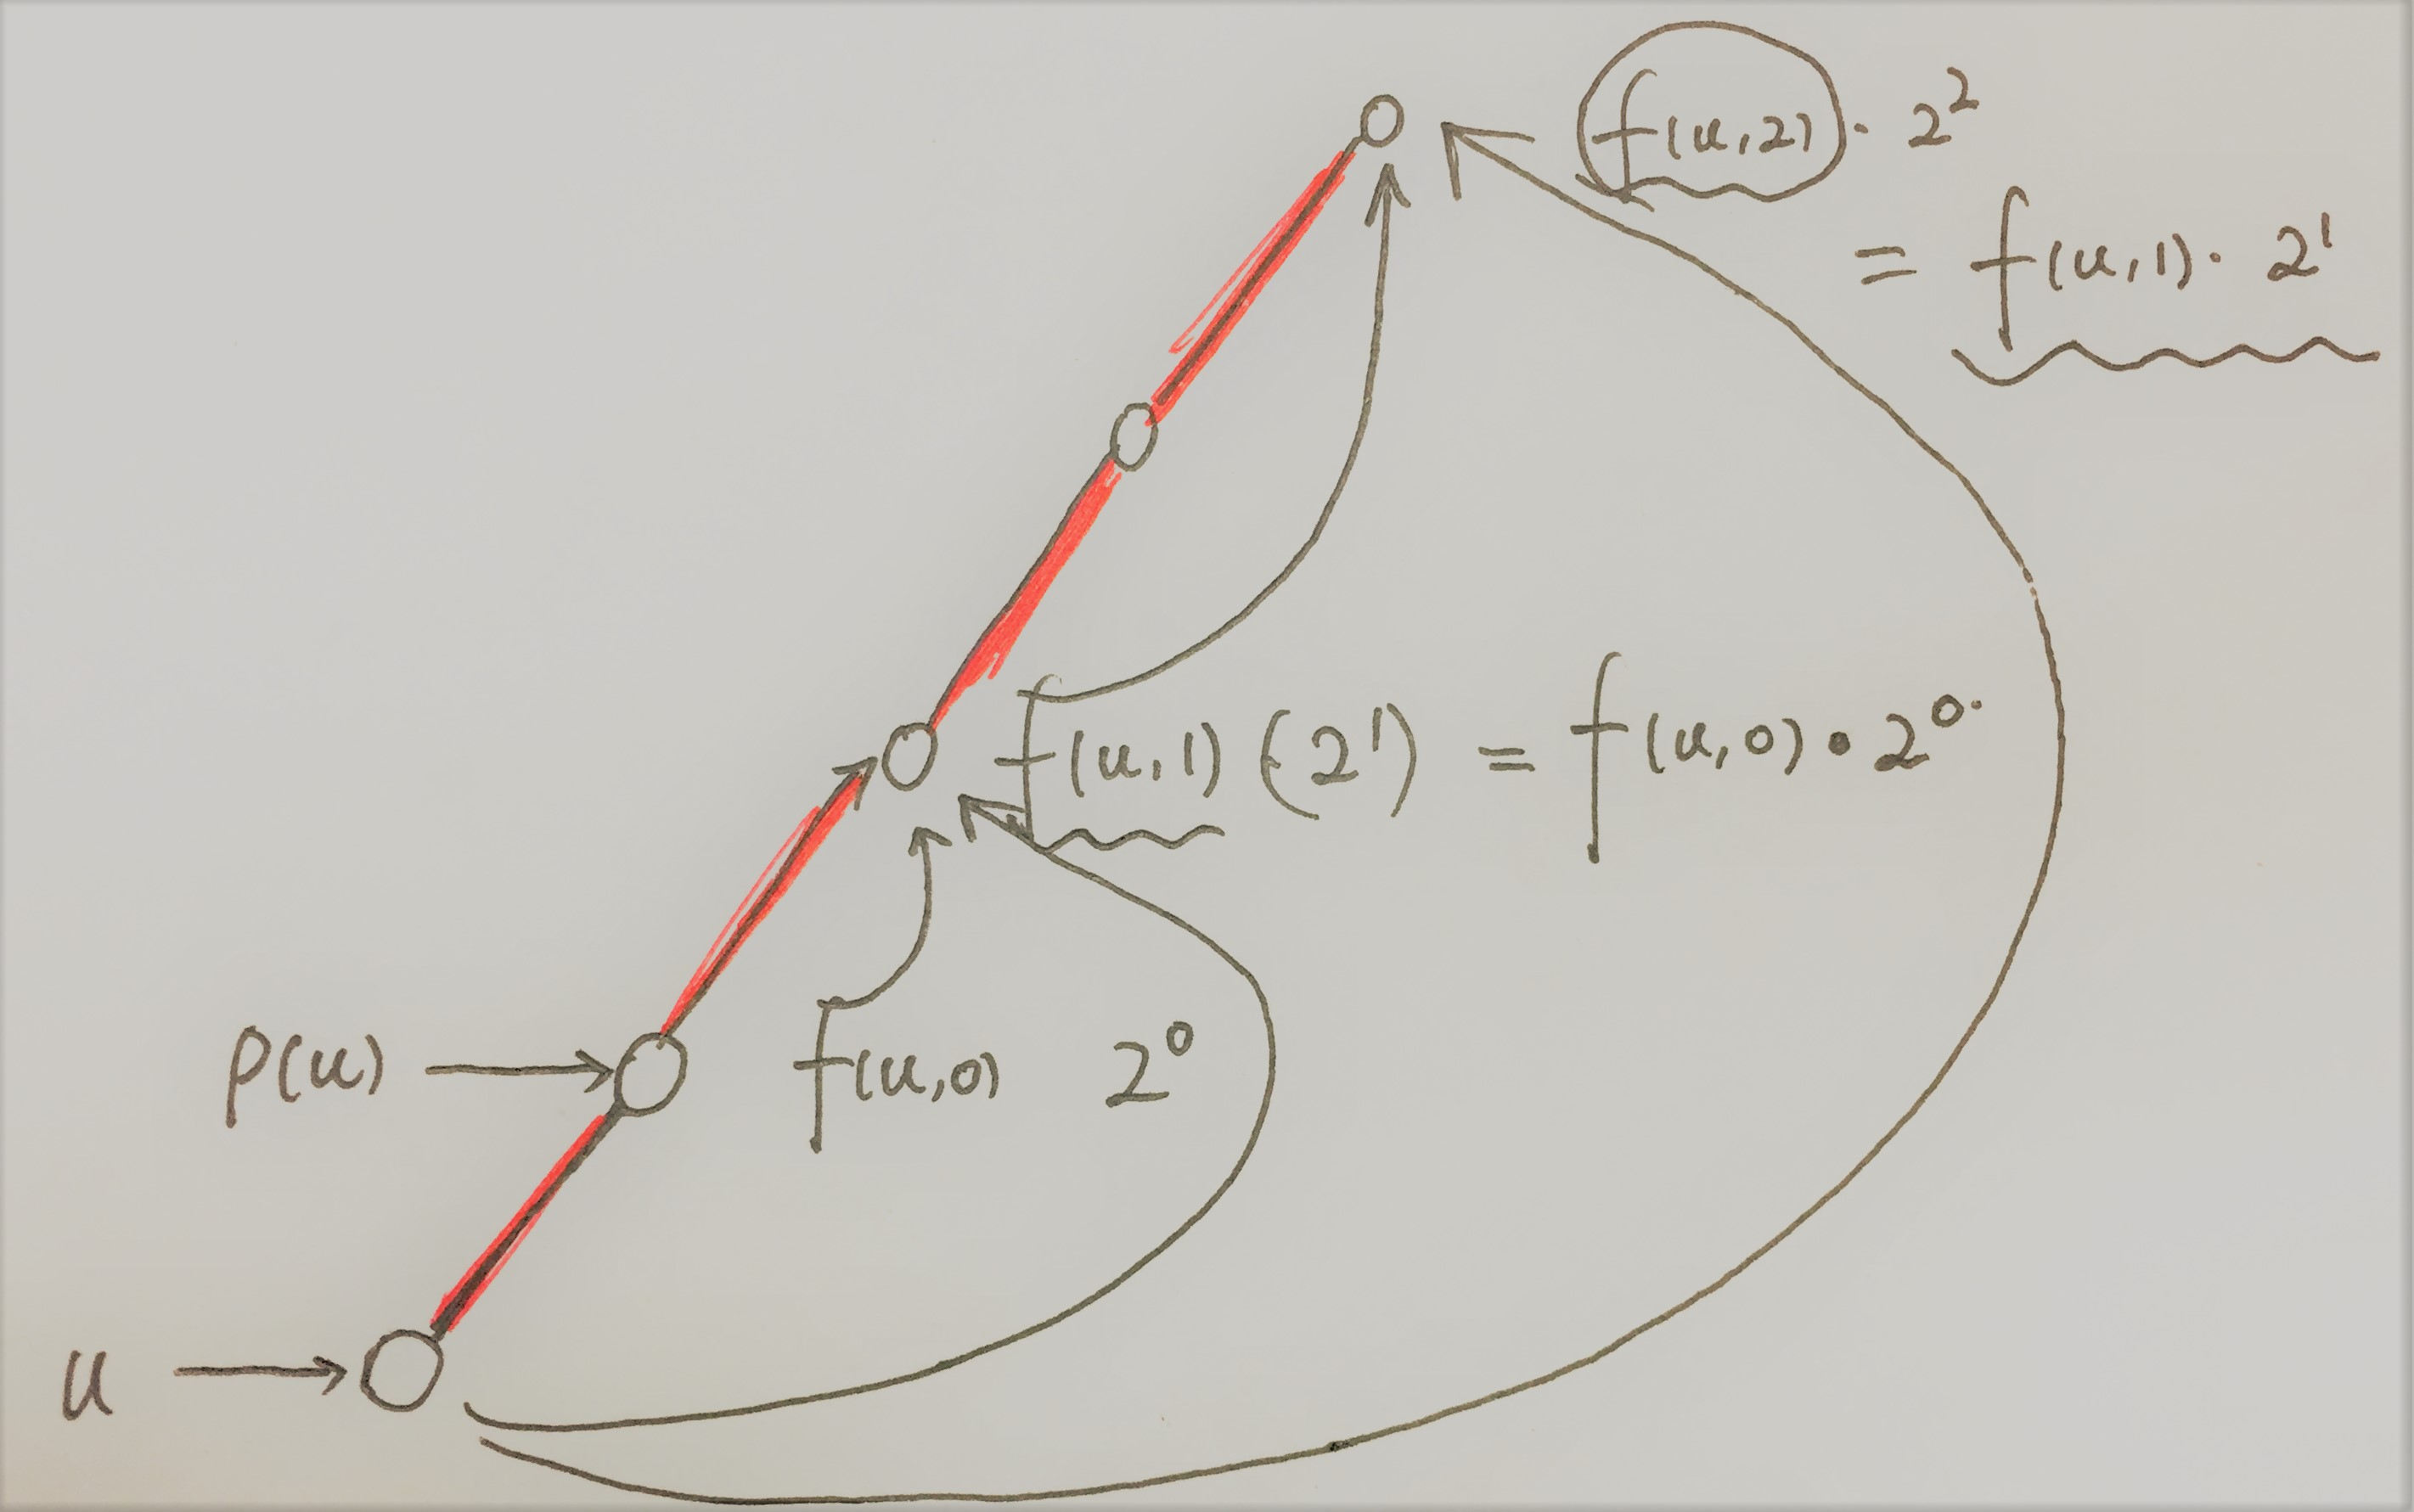
\includegraphics[width=.4\textwidth]{./fig/IMG_6072.JPG}
	\end{figure}
	
	So now it is clear this is true because:
	\[ 2^{i} = 2^{i-1}+2^{i-1} \]
\end{enumerate}
Now let's see the code:
\begin{lstlisting}[language=C++]
L[0]=-1;L[1] = 0; f[1,0]=1; // Initialize: root=1 with level 0 
dfs(1,0);
void dfs( int root, int level ){
	L[root] = level; int tl = level; 
	nodes[ root ].visited = true; 
	
	for( int i = 1; (tl >> i) ; i ++ )
		f[ root ][i] = f[ f[root][i-1] ][ i-1 ]; // Visit after its ancestors have been visited.

	for( int i = 0; i < mst[root].size() ; i ++ ){
			int next = tree[root][i];
			if( !nodes[next].visited ){
				f[ next ][0] = root; // Initialize: direct ancestor 
				dfs( next, level+1 ); // With level+1 compared with its parent
			}
	}
	return;
}
\end{lstlisting}

Many things could be done by the $f$ matrix. Let's give some examples:

(1). Longest path along two nodes $x,y$ to their LCA:
\begin{lstlisting}[language=C++]
int lca( int x, int y ){
	if( L[y] > L[x] )
		swap(x,y);  // Make sure x is lower
	
	int res = 0;
	for( int i = 19; i >= 0; i -- ) // 19 > log(n), pre-defined
		if( L[ f[x][i] ] >= L[y] ){ // Still lower than y
			res = max( res,dis[x][i] ); // Information along the path
			x = f[x][i]; // Notice in the next iteration, i->i-1
			// No break here!
		}
	
	if( x == y ) return res;

	for( int i = 19; i >= 0; i -- ){
		if( f[x][i] != f[y][i] ){
			res = max( res,max( dis[x][i],dis[y][i] ) );
			x = f[x][i];
			y = f[y][i];
		}
	}

	return max( res, max( dis[x][0],dis[y][0] ) );
}
\end{lstlisting}
Some explainations:
\begin{itemize}
	\item $res$ matrix, this can be done by the same way of $f$:
	\[
			res[u,i] =\left\{ \begin{array}{ll}
				w(u,p(u)),& \text{if }i=0\\
				\\
				\max (res[u,i-1],res[ f[u,i-1],i-1 ]),&\text{otherwise}
			\end{array}
		\right.
	\]
	\item row 6-11: this is the key. To make it clear,
	\begin{itemize}
		\item[-] $L[f[x,19]]$ is surely less than $L[y]$.
		\item[-] The very first $i$ to make $L[f[x,i]] \ge L[y]$ has two meanings: (1). this node is below than $y$; (2). $f[ f[x,i],i ]$ is upper than $y$. But we don't know $f[ f[x,i],i-1 ]$. This is what the codes done next, to check $L[ f[x,i],i-1 ]$. 
		\item[-] Finally, when $i=0$, we'll get a node having the same level of $y$, cause $i=1$ check the nodes two levels above, $i=0$ check the nodes above.
	\end{itemize}
	\item The remain things are simple. Row 15-21, $x,y$ always have the same level.
\end{itemize}

(2). Longest edge along the path to root. Just let $y=1$,...

(3). Almost everything could be done for answering queries about the dfs path on trees.


\subsection*{Some problems}
\begin{itemize}
	\item \href{http://codeforces.com/problemset/problem/609/E}{609E. Minimum spanning tree for each edge}
	\item \href{http://codeforces.com/contest/733/problem/F}{733F. Drivers dissatisfaction}
	\item \href{http://codeforces.com/problemset/problem/739/B}{739B. Alyona and a tree}
\end{itemize}

\newpage
\subsection*{Tutorial of 739B}
There's two key parts of this problem:
\begin{itemize}
	\item Binary lifting to document and query the path
	\item Partial sum on trees for answering questions
		\[ dist[u,v] = depth[v]-depth[u] \]
\end{itemize}

During binary lifting or binary search, a most important care of the bound defintion, for example $lower\_bound$ or $upper\_bound$.In this problem, $upper\_bound$ may be appropriate. We document the first ancestor which can not control one node.

Then for one node, the answer can be right:
\[ ans[r]=\sum_{child_i}(ans[child_i]+1)-no[r] \]
where $no[r]$ documents the number of nodes ending on $r$.

\vspace{20pt}

\bf Reference: \url{http://codeforces.com/blog/entry/22325}
\end{document}
